%*******************************************************************************
%****************************** Chapter Three **********************************
%*******************************************************************************
\chapter{Nonlinear Analysis} \label{chapter3}

%****************************** Define Graphics Path ***************************
%\ifpdf
%    \graphicspath{{chapter4/figs/raster/}{chapter4/figs/PDF/}{chapter4/figs/}}
%\else
%    \graphicspath{{chapter4/figs/vector/}{chapter4/figs/}}
%\fi
%
\graphicspath{{figs/chapter3/PDF/}}

\section{Introduction}
Nonlinear analysis investigate the dynamics of observed time-ordered data.
Methods of nonlinear analysis, for this thesis, entail determination 
of embedding parameters, state space reconstruction, uniform time-delay
embedding, recurrence plots and recurrence quantification analysis. 

The method of state space reconstruction was originally proposed by 
\cite{packard1980} and formalised by \cite{takens1981}. Since then, various 
investigations and disciplines relative to nonlinear time series analysis 
have benefited from it \citep{aguirre2009, stergiou2011, frank2010, sama2013}.
The method of reconstructed state space (RSS) is based on uniform time-delay 
embedding (UTDE) which is a simple matrix implementation considering the 
embedding 
parameters ($m$ and $\tau$), therefore, matrix represents the reconstruction
of an unknown $d-$dimensional manifold $M$ from a scalar 
time series (e.g. one-dimensional time series in $\mathbb{R}$).
A manifold, in this context, is a multidimensional curved surface within a 
space (e.g. a saddle) \citep{guastello-gregson2011}.
Henceforth, the method of state space reconstruction using a scalar time series 
can preserve dynamic invariants such as correlation dimension, 
fractal dimension, Lyaponov exponents or Kolmogorov-Sinai entropy 
\citep{bradley2015, Quintana-Duque2012, 
Quintana-Duque2013, Quintana-Duque2016, krakovska2015}.
However, 
there are still many challenging research questions to be answered  
with regards to the selection of appropriate embedding parameters 
that preserver the dynamics of a system 
for the computation of methods nonlinear analysis such as RSS, RPs and RQAs.
With that in mind, the following methods are described in this chapter: 
the state space reconstruction theorem (RSSs), 
uniform time-delay embedding theorem (UTDE), and
methods to compute embedding parameters: 
false nearest neighbours (FNN)
and average mutual information (AMI).
Additionally, fundamentals of Recurrence plots(RPs), 
Recurrence quantification analysis (RQA)
and the introduction of 3D surface plots of RQA
are presented in this chapter.

\section{State Space Reconstruction Theorem} \label{sec:rss}
Following the notation employed in \cite{casdagli1991, garland2016, 
gibson1992, uzal2011, uzal2010, takens1981}, the method of state space 
reconstruction is defined by:
%%********************************[EQUATION]************************************
\begin{equation}\label{eq:ssr}
  s(t)=f^t [s(0)],
\end{equation}
%%********************************[EQUATION]************************************
where $s$, $s: A \rightarrow M$ given that $A \subseteq \mathbb{R}$ and $M 
\subseteq \mathbb{R}^d$, represents a trajectory which evolves in an 
unknown $d-$dimensional manifold $M$, $f: M \rightarrow M$ is an evolution 
function and $f^t$, with time evolution $t \in \mathbb{N}$, is the $t$-th 
iteration of $f$ that corresponds to an initial position $s(0) \in M $ 
\citep{takens1981}.
Then, a point of a scalar time series $x(t)$ in $\mathbb{R}$, can be obtained 
with
%%********************************[EQUATION]************************************
\begin{equation}\label{eq:measurement}
	x(t)=h[s(t)],
\end{equation}
%%********************************[EQUATION]************************************
where $h$ is a function, $h: M \rightarrow \mathbb{R}$, defined on the 
trajectory $s(t)$.

Reconstructed state space can then be described as an $n-$dimensional state 
space defined by $y(t)=\Psi[\boldsymbol{X}(t)]$ where 
$\boldsymbol{X}(t) = \{ x(t), x(t-\tau) , ...,x(t - (m-1)\tau  ) \}$ is the 
uniform time-delay embedding with a dimension embedding $m$ and delay 
embedding $\tau$ and $ \Psi: \mathbb{R}^m \rightarrow \mathbb{R}^n$ is a 
further transformation of dimensionality (e.g. Principal Component Analysis, 
Singular Value Decomposition, etc) being $n \leq m$. With that in mind, 
uniform time-delay embedding, $\boldsymbol{X}(t)$, defines a map 
$\Phi: M \rightarrow \mathbb{R}^m$ such that $\boldsymbol{X}(t) = \Phi(s(t))$,
where $\Phi$ is a diffeomorphic map \citep{takens1981} whenever $\tau > 0$ 
and $m > 2d_{box}$ and $d_{box}$ is the box-counting dimension of 
$M$ \citep{garland2016}.
Then, if $\Phi$ is an embedding of an attractor (i.e. evolving 
trajectories) in the reconstructed state space, a composition of functions 
represented with $F^t$ is induced on the reconstructed state space:
%********************************[EQUATION]************************************
\begin{equation}\label{eq:st}
  \boldsymbol{X}(t)=F^t [\boldsymbol{X}(0)] = \Phi \circ f^t \circ \Phi ^{-1}[\boldsymbol{X}(0)].
\end{equation}
%%********************************[EQUATION]************************************
Hence, an embedding is defined as "a smooth one-to-one coordinate 
transformation with a smooth inverse" \citep[p. 54]{casdagli1991}. 
Figure~\ref{fig:ssr} illustrates the state space reconstruction.
%---------------------------------(FIGURE)-------------------------------------
\begin{figure}
  \centering
    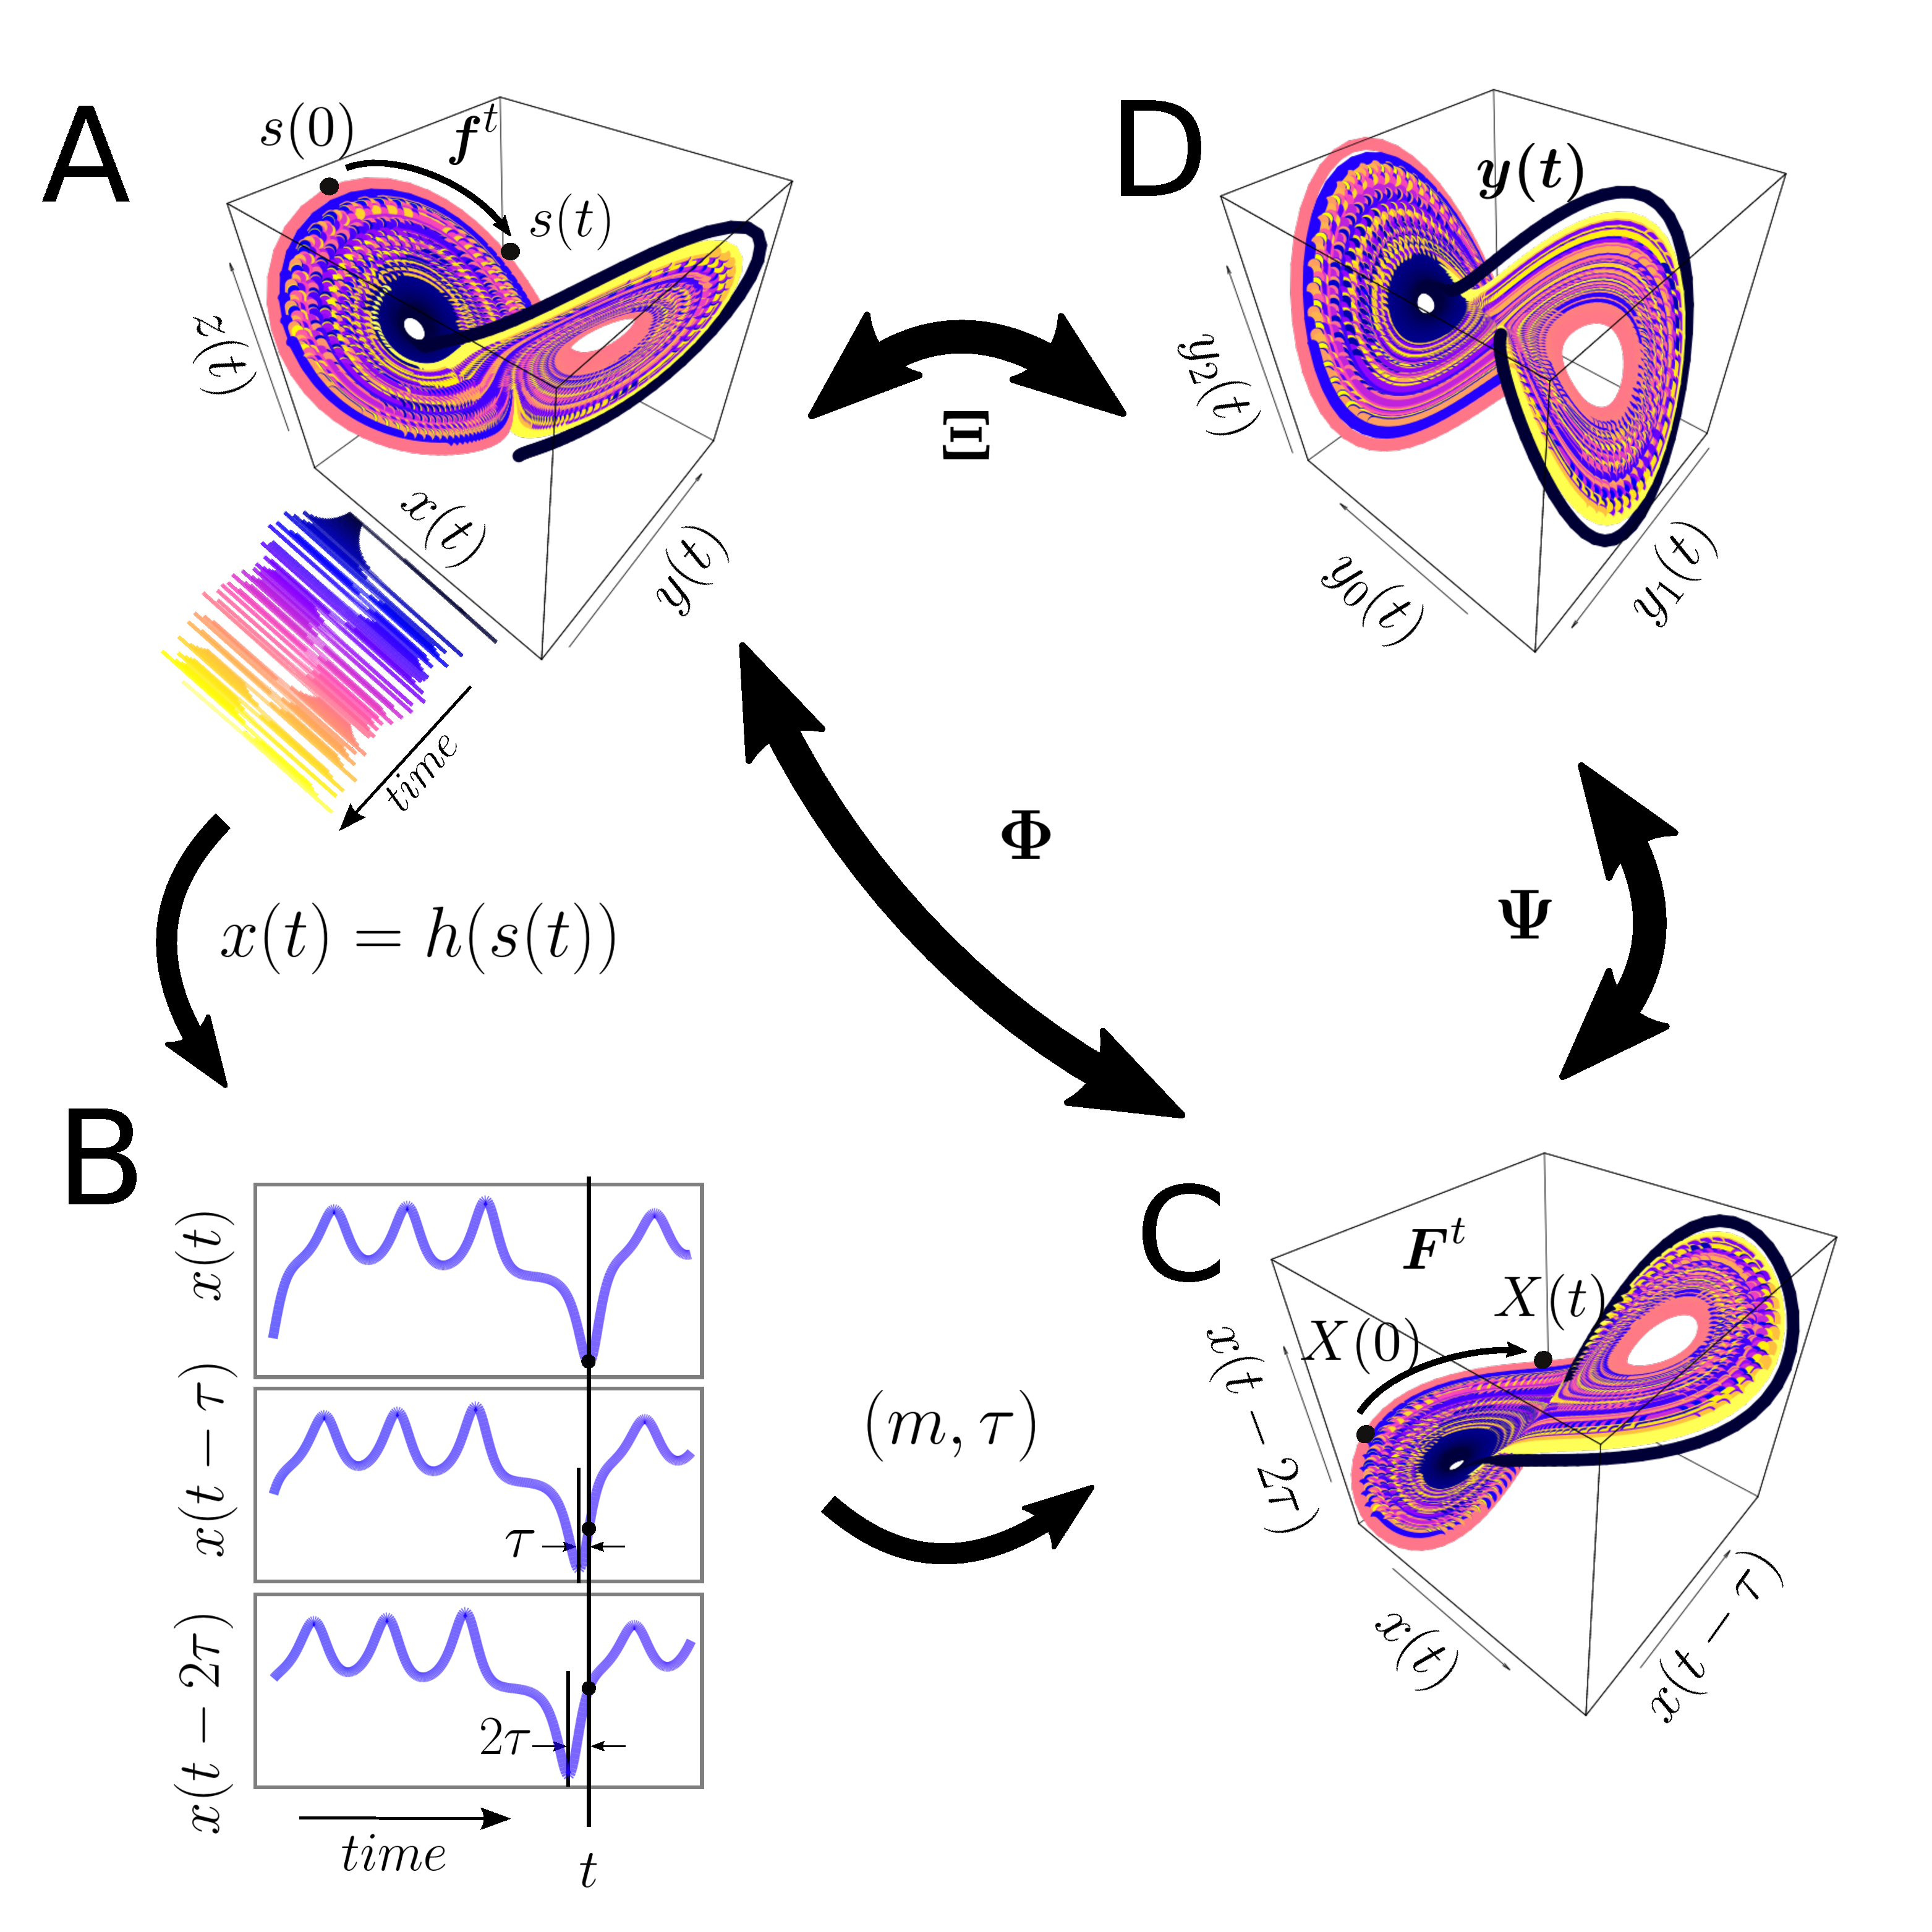
\includegraphics[width=0.95\textwidth]{fig_3_01}
    \caption[State space reconstruction methodology]{
	{\bf State space reconstruction methodology.}
	State space reconstruction is based on $x(t)=h[s(t)]= h[f^t [s(0)]]$
	where $h[ ]$ is a function $h: M \rightarrow \mathbb{R}$, defined on 
	the trajectory $s(t)$. $f$ is the true dynamical system, 
	$f:M \rightarrow M$, defined as evolution function and $f^t$, 
	with time evolution $t \in \mathbb{N}$ which is the $t$-th iteration 
	of $f$ that corresponds to an initial position $s(0) \in M $. 
	The time-delay embedding represented as $\Phi$, maps the original
    	$d-$dimensional state $s(t)$ into the $m-$dimensional uniform 
	time-delay embedding matrix $\boldsymbol{X}(t)$.
	The transformation map $\Psi$ maps $\boldsymbol{X}(t)$ into a 
	new state space $y(t)$ of dimensions $n < m$.
	(A) $M-$dimensional state space (e.g. Lorenz system);
    	(B) Delayed copies of $1-$dimensional $x(t)$ from the Lorenz system;
    	(C) $m-$dimensional reconstructed state space with 
	\texorpdfstring{$m$}{m} and    \texorpdfstring{$\tau$}{T}, and 
    	(D) $y(t)$ is the $n-$dimensional reconstructed state space.
	The total reconstruction map is represented as $\Xi = \Psi \circ \Phi $
	where $\Phi$ is the delay reconstruction map and 
	$\Psi$ is the coordinate transformation map.
	This figure is adapted from the work of 
   	\cite{Quintana-Duque2012, casdagli1991, uzal2011}.
	\R code to reproduce the figure is available at 
	\codelink{
	https://github.com/mxochicale/phd-thesis/tree/master/0_code_data/1_code/4_figs_ch3/fig_3.1/code
	}.
    }
    \label{fig:ssr}
\end{figure}
%%---------------------------------(FIGURE)-------------------------------------

\section{Uniform Time-Delay Embedding (UTDE)}\label{sec:utimedelayembedding}
\cite{frank2010} and \cite{sama2013} refer to the state space reconstruction 
outlined in \ref{sec:rss} as "time-delay embeddings" or "delay coordinates", 
respectively. However, the term "uniform time-delay embedding" 
is considered as being more descriptive and appropriate terminology 
for this thesis.

The uniform time-delay embedding is represented as a matrix of uniform 
delayed copies of the time series $\{ \boldsymbol{x}_n \}_{n=1}^N$ where $N$ 
is the sample length of $\{ \boldsymbol{x}_n \}$ and $n$ is index for the 
samples of $\{ \boldsymbol{x}_n \}$. $\{ \boldsymbol{x}_n \}_{n=1}^N$ has a 
sample rate of $T$. The delayed copies of $\{ \boldsymbol{x}_n \}$ are 
uniformly separated by $\tau$ and represented as 
$\{\boldsymbol{ \tilde{x} }_{n- i\tau} \}$ where $i$ goes from 
$0,1, \dots, (m-1)$ (Fig~\ref{fig:utde}).
$\{\boldsymbol{ \tilde{x} }_{n- i\tau} \}$ contains information of unobserved 
state variables and encapsulates the information of the delayed copies of 
the available time series in the uniform time-delay embedding matrix 
$\boldsymbol{X}^{m}_{\tau}$, $\boldsymbol{X}^{m}_{\tau} \in \mathbb{R}^m$, 
defined as
%%********************************[EQUATION]************************************
\begin{equation}\label{eq:tde}
\boldsymbol{X}^{m}_{\tau}  =
\begin{pmatrix}
\boldsymbol{ \tilde{x} }_n \\
\boldsymbol{ \tilde{x} }_{n-\tau} \\
\boldsymbol{ \tilde{x} }_{n-2\tau} \\
\vdots \\
\boldsymbol{ \tilde{x} }_{n- (m-1) \tau} \\
\end{pmatrix}^\intercal, 
\end{equation}
%%********************************[EQUATION]************************************
where $m$ is the embedding dimension, $\tau$ is the embedding delay and
$ ^\intercal$ denotes the transpose. $m$ and $\tau$ are known as embedding 
parameters.
%%%********************************[EQUATION]************************************
The matrix dimension of $ \boldsymbol{X}_{\tau}^{m} $ is defined by
$N-(m-1)\tau$ rows and $m$ columns and $N-(m-1)\tau$ defines the length of 
each delayed copy 
of $\{ \boldsymbol{ \tilde{x} }_n \}$ in $\boldsymbol{X}^{m}_{\tau}$.
A graphical representation of uniform time-delay embedding is shown in 
Figure~\ref{fig:utde}. See Appendix \ref{appendix:a} for further details 
and explicit examples of uniform time-delay embedding methodology. 
%---------------------------------(FIGURE)-------------------------------------
\begin{figure}
 \centering
   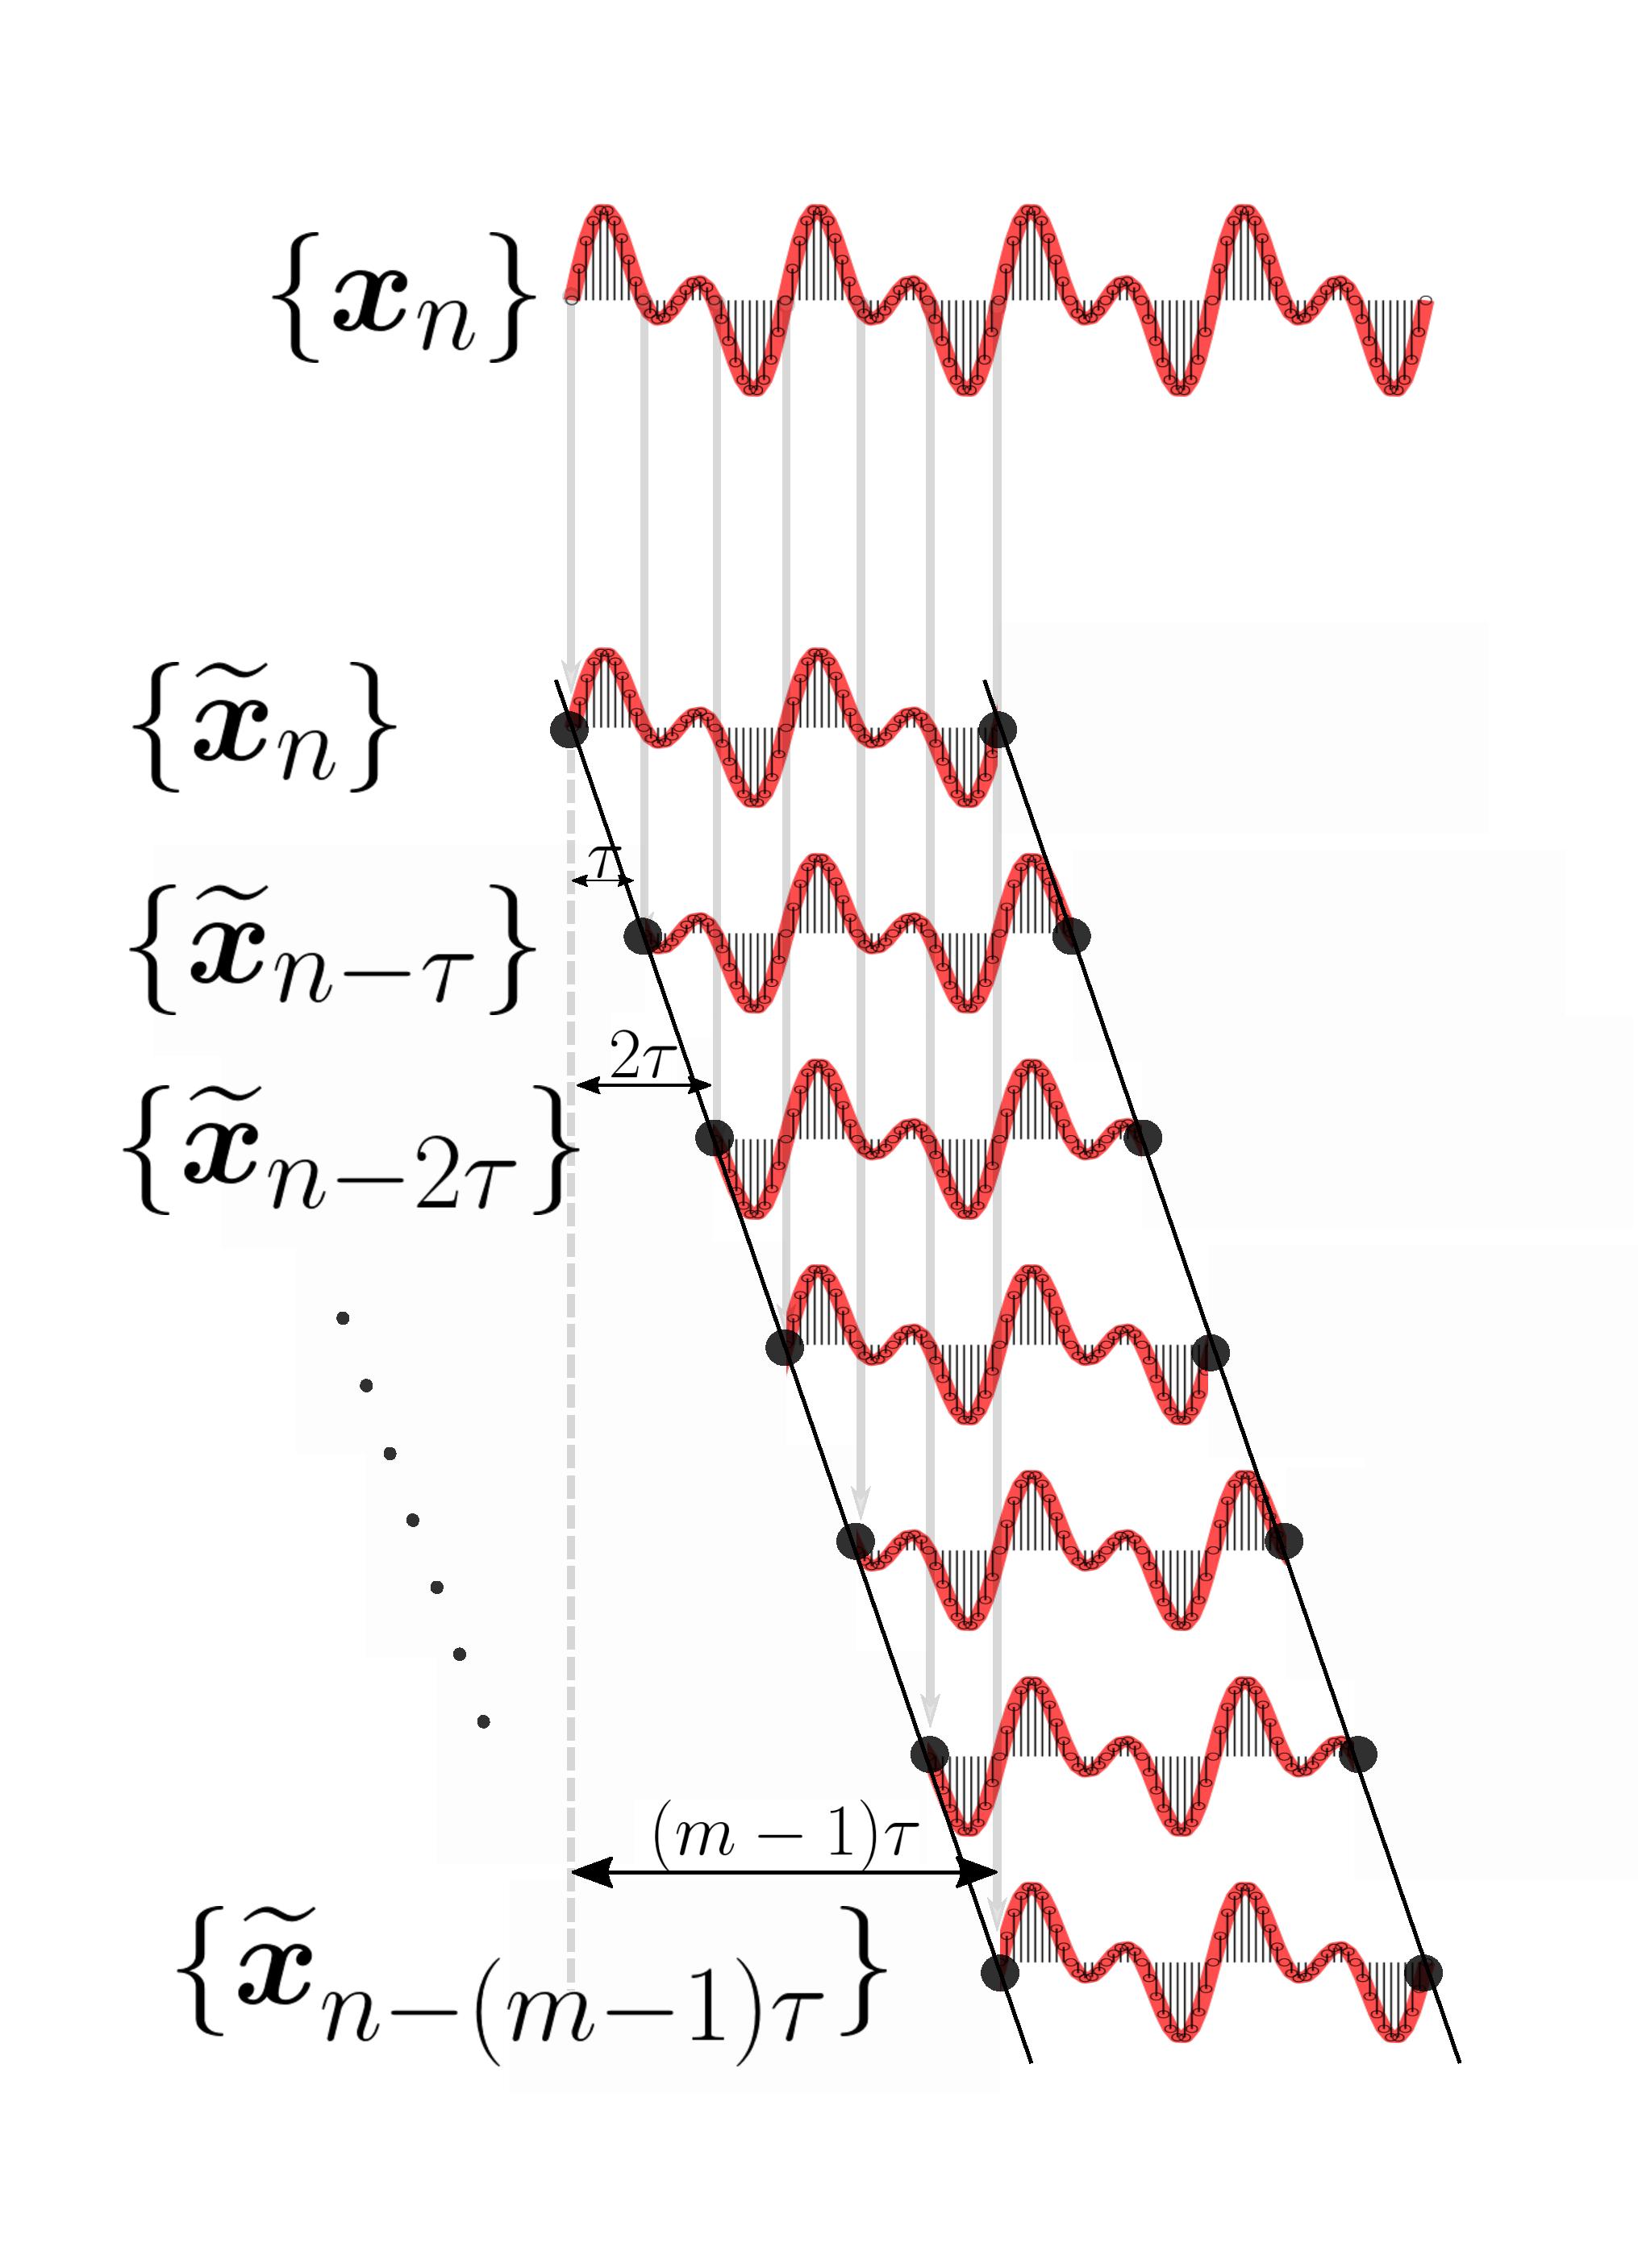
\includegraphics[width=0.95\textwidth]{fig_3_02}
   \caption
	[Uniform time-delay embedding]{
	{\bf Uniform time-delay embedding (UTDE).} 
	UTDE is illustrated as $m-1$ delayed copies
   	of $\{ \boldsymbol{x}_n \}$ which is uniformly separated by $\tau$.
	UTDE is represented as
	$\{ \boldsymbol{ \tilde{x} }_n, \dots,  
	\boldsymbol{ \tilde{x} }_{n -(m-1)\tau}   \}$ (Eq.~\ref{eq:tde}).
	\R code to reproduce the figure is available at 
	\codelink{
	https://github.com/mxochicale/phd-thesis/tree/master/0_code_data/1_code/4_figs_ch3/fig_3.2/code
	}.
   }
   \label{fig:utde}
\end{figure}
%%---------------------------------(FIGURE)-------------------------------------

\section{Estimation of Embedding Parameters}
The estimation of the embedding parameters ($m$ and $\tau$) is an essential 
step for the state space reconstruction in order to apply the method of
uniform time-delay embedding (UTDE). 
Hence, two of the most common algorithms are reviewed, 
which will be used in this thesis, to compute the embedding
parameters: the false nearest neighbour (FNN) and the average mutual 
information (AMI).

\subsection{False Nearest Neighbours (FNN)} \label{ch3:fnn}
To select the minimum embedding dimension $m_0$, \cite{kennel1992}
used the method of false neighbours which can be understood as follows:
on one hand, when the embedding dimension is too small to unfold the attractor
(i.e. evolving trajectories in a state space) 
"not all points that lie close to each other will be neighbours and some points
appear as neighbours as a result of the attractor being projected down into an
smaller space", on the other hand, when increasing the embedding dimension 
"points that are near to each other in the sufficient embedding dimension 
should remain close as the dimension increase from $m$ to $m+1$"
\citep[p. 3]{krakovska2015}.

From a mathematical point of view, state space reconstruction is done when 
the attractor is unfolded with either the minimum embedding dimension, $m_0$, 
or any other embedding dimension value where $m \ge m_0$ \citep{kennel1992}.
In contrast, any large value of $m_0$ leads to excessive computations 
\citep{bradley2015}. Hence, \cite{Cao1997} proposed an algorithm based on the
false neighbour method where only the time-series and one delay embedding value 
are necessary to select the minimum embedding dimension. 
Cao's algorithm is based on $E(m)$, which is the mean value of all $a(i,m)$,
and defined as: 
%%********************************[EQUATION]************************************
\begin{equation}\label{eq:e}
  \begin{aligned}
E(m) &= \frac{1}{N-m\tau} \sum_{i=1}^{N-m\tau} a(i,m) \\
    &=
       \frac{1}{N-m\tau} \sum_{i=1}^{N-m\tau}
       \frac{ || \boldsymbol{X}_i(m+1) - \boldsymbol{X}_{n(i,m)}(m+1) || }
            { || \boldsymbol{X}_i(m) - \boldsymbol{X}_{n(i,m)}(m) ||  }
  \end{aligned}
\end{equation}
%%********************************[EQUATION]************************************
where $\boldsymbol{X}_i(m)$ and $\boldsymbol{X}_{n(i,m)}(m)$ are uniform time-delay
embeddings with $i=1,2,\dots,N-(m-1)\tau$ and 
$ n(i,m)= 1 \le n(i,m) \le N-m\tau$.
From Eq.~\ref{eq:e} $E(m)$ is only dependent on $m$ and $\tau$ for which 
$E_1(m)$ is defined as
%%********************************[EQUATION]************************************
\begin{equation}\label{eq:e1}
E_1(m) = \frac{ E(m+1) } { E(m)}.
\end{equation}
%%********************************[EQUATION]************************************
$E_1(m)$ is therefore proposed to describe the variation from $m$ to $m+1$
in order to find the minimum embedding dimension $m_0$ (Eq.~\ref{eq:e1}).
As \citealt[p. 44]{Cao1997} described: "$E_1(m)$ stops changing when $m$ is 
greater than some $m_0$, if the time series comes from a multidimensional 
state space then $m_0 + 1$ is the minimum dimension".
Additionally, \cite{Cao1997} proposed $E_2(m)$ to distinguish deterministic 
signals from stochastic signals. $E_2(m)$ is defined as
%%********************************[EQUATION]************************************
\begin{equation}\label{eq:e2}
E_2(m) = \frac{ E^* (m+1) } { E^*(m)},
\end{equation}
%%********************************[EQUATION]************************************
where
%%********************************[EQUATION]************************************
\begin{equation}\label{eq:ee}
E^*(m) = \frac{1}{N-m\tau} \sum_{i=1}^{N-m\tau}
|| \boldsymbol{X}_i(m+1) - \boldsymbol{X}_{n(i,m)}(m+1) ||.
\end{equation}
%%********************************[EQUATION]************************************
For instance, when the signal comes from random noise (values that are 
independent from each other), all $E_2(m)$ values are approximately equal 
to 1 (e.g. $E_2(m) \approx 1$). However, for deterministic data $E_2(m)$ is 
not constant for all $m$ (e.g. $E_2(m) \neq 1$).

Two time series are considered as an example of the 
use of $E_1(m)$ and $E_2(m)$ values, 
the solution for the $x$ variable  of the chaotic deterministic Lorenz 
system (Figure~\ref{fig:e1e2}E), and a Gaussian noise time series with 
zero mean and a variance of one (Figure~\ref{fig:e1e2}F).
Then $E_1(m)$ and $E_2(m)$ values are computed for each time series.
The $E_1(m)$ values for the chaotic time series appear to be constant
after the dimension is equal to six. The determination of six is 
given that any value of $m$ can be used as $E_1(m)$ values are within 
the threshold of $1\pm0.05$ (Fig~\ref{fig:e1e2}A). 
Althought the $E_2(m)$ values for the chaotic time series tend to be closer to
one as $m$ increses, these are different to one (Fig~\ref{fig:e1e2}C), 
for which, it can be concluded that the chaotic time series comes 
from a chaotic deterministic signal.
With regard to the noise time series,  $E_1(m)$ values appeared to be constant
when $m$ is close to thirteen which is defined by the same threshold of 
$1\pm0.05$ (Figure~\ref{fig:e1e2}B). 
Then, contrary to the $E_2(m)$ values for a chaotic 
Lorenz time series, all values of $E_2(m)$ for a noise time series are 
approximately equal to one (Figure~\ref{fig:e1e2}D). 
Hence, $E_1(m)$ values then indicate the minimum 
embedding dimension of the noisy time series is thirteen, however all of 
the $E_2(m)$ values are approximately equal to one (Figure~\ref{fig:e1e2}D),
for which, it can be concluded that noise time series is a stochastic signal.
%%---------------------------------(FIGURE)-------------------------------------
\begin{figure}[!h]
  \centering
  \includegraphics[width=1.0\textwidth]{fig_3_03}
    \caption
	[Minimum dimension embedding values with Cao's method]{
	{\bf Minimum dimension embedding values with Cao's method.} 
	(A, B) $E_1 (m)$ values and (C, D) $E_2(m)$ values 
	with variations of $\tau$ values from one to twenty
	for (E) chaotic and (F) random time series.
	\R code to reproduce the figure is available at 
	\codelink{
	https://github.com/mxochicale/phd-thesis/tree/master/0_code_data/1_code/4_figs_ch3/fig_3.3/code	
        }.
	}
    \label{fig:e1e2}
\end{figure}
%%---------------------------------(FIGURE)-------------------------------------

It is important to note that for this thesis not only the values for 
$E_1(m)$ and $E_2(m)$ are computed but also a variation of $\tau$ from 
1 to 20 (Figure~\ref{fig:e1e2} (A,B,C,D)) has been explored. 
The purpose of using variations for $\tau$ is to show its independence 
with regard to the $E_1(m)$ (Fig. \ref{fig:e1e2}(A,B))
and $E_2(m)$ (Fig. \ref{fig:e1e2}(C,D)).
Although \cite{Cao1997} mentioned that no parameters are required to find
the minimum embedding dimension, it has been found, in this thesis, 
that it is necessary to define a threshold for which $E_1(m)$ values 
appear to be constant. 
Hence, for the given examples and the reported results for this thesis,
a threshold of 0.05 is defined (see Fig. \ref{fig:e1e2}(A) 
with the parallel lines of the threshold near to one $1\pm0.05$).
Additionally, see optimal embedding parameters on
Chapter \ref{chapter7} for further research regarding the 
selection of such threshold.


\subsection{Average Mutual Information (AMI)}
One would experience the following when selecting 
the delay dimension parameter, $\tau$:
(i) when $\tau$ is too small, the elements of uniform time-delay embedding will be 
along the bisectrix of the phase space and the reconstruction is generally 
not satisfactory, 
(ii) when $\tau$ is too large the elements of the uniform 
time-delay embedding will become spread and uncorrelated which makes 
recovering the underlying attractor (i.e. evolving trajectories in a 
state space) difficult, if not impossible 
\citep{casdagli1991, emrani2014a, garcia2005e71}.

There are many approaches to compute the embedding parameters 
\citep{bradley2015}, for instance, geometry-based methodologies where 
the amount of space filled in the reconstructed state is the metric to 
compute the delay embedding \citep{mrosenstein1994} or 
theoretical approaches to estimate an optimal parameter for 
$\tau$ \citep{casdagli1991}. 
However, the autocorrelation function and the average mutual information 
(AMI) are the two most commonly used algorithms to compute the minimum 
delay embedding parameter $\tau_0$. \cite{emrani2014a} used the 
autocorrelation function in which the first zero crossing is considered 
as the minimum delay embedding parameter. However, the autocorrelation 
function is a linear statistic whereas AMI considers the nonlinear 
dynamical correlations \citep{afraser1986,krakovska2015}.
With that in mind, the AMI algorithm is described below to estimate 
the minimum delay embedding parameter, \texorpdfstring{$\tau_0$}{T}.

To compute the AMI, an histogram of $x(n)$ using $n$ bins is calculated
and then a probability distribution of data is computed \citep{kantz2003}.
AMI is therefore denoted by $I(\tau)$ which is the average mutual 
information between the original time series, $x(n)$, and the delayed time 
series, $x(n-\tau)$, delayed by $\tau$ \citep{kabiraj2012}. AMI is defined by
%%********************************[EQUATION]************************************
\begin{equation}\label{eq:ami}
I(\tau) = \sum_{i,j}^N p_{ij} \log_2 \frac{ p_{ij} }{ p_i p_j },
\end{equation}
%%********************************[EQUATION]************************************
where probabilities are defined as follows: 
$p_i$ is the probability that $x(n)$ has a value inside the $i$-th bin of 
the histogram, $p_j$ is the probability that $x(n+\tau)$ has a value inside 
the $j$-th bin of the histogram and $p_{ij}(\tau)$ is the probability 
that $x(n)$ is in bin $i$ and $x(n+\tau)$ is in bin $j$.
The AMI is measured in bits (base 2, also called shannons) 
\citep{kantz2003, nonlinearTseries2016}.
For small $\tau$ ($\tau < 3$), AMI will be large ($I(\tau)>6$) and as 
$m$ increase AMI will then decrease rapidly. Hence, as $\tau$ increase 
and goes to a large limit, $x(n)$ and $x(n+\tau)$ have 
nothing to do with each other and $p_{ij}$ is factorised as $p_ip_j$ for 
which AMI is close to zero.  Then, in order to obtain $\tau_0$, 
"it has to be found in the first minimum of $I(\tau)$ where $x(n+\tau)$ 
adds maximal information to the knowledge from $x(n)$" meaning that the 
redundancy between $x(n+\tau)$ and $x(n)$ is the least
\citep[p. 151]{kantz2003}.

%%---------------------------------(FIGURE)-------------------------------------
\begin{figure}[!h]
  \centering
  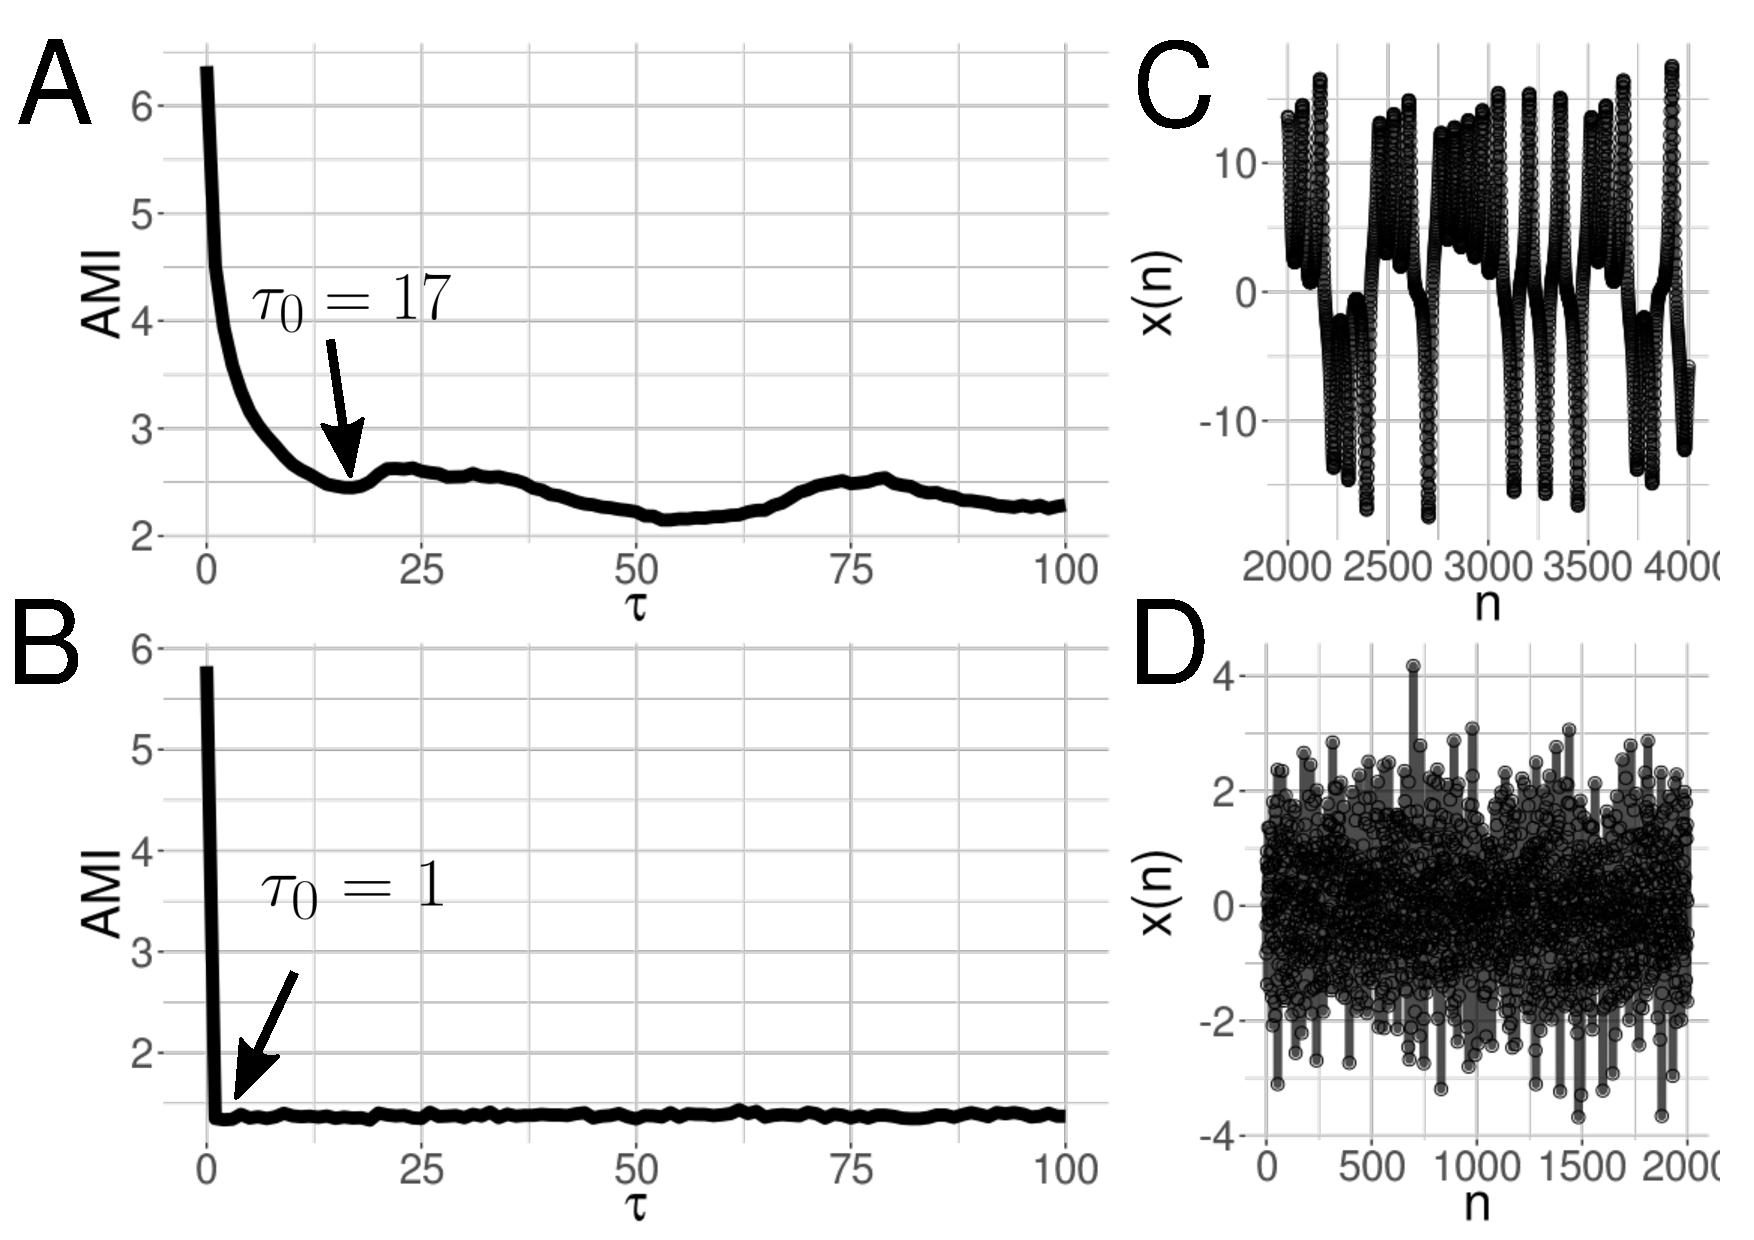
\includegraphics[width=0.7\textwidth]{fig_3_04}
    \caption
	[Minimum delay embedding values with AMI's method]{
	{\bf Minimum delay embedding values with AMI's method.} 
    	(A, B) AMI values where its first minimum value in the curve
	is the minimum time delay embedding ($\tau_0$), 
	for (C) a chaotic and (D) noise time series.
	\R code to reproduce the figure is available at 
	\codelink{
	https://github.com/mxochicale/phd-thesis/tree/master/0_code_data/1_code/4_figs_ch3/fig_3.4/code	
        }.
        }
    \label{fig:amis}
\end{figure}
%%---------------------------------(FIGURE)------------------------------------
For example, the AMI is computed for two time series:
(i) the $x$ solution of the deterministic chaotic Lorenz system, and 
(ii) a noise time series using a normal distribution with mean zero and 
standard deviation equal to one. The AMI plots are shown in 
Figure~\ref{fig:amis}, where the minimum delay embedding parameter for 
the chaotic time series is $\tau_0=17$ and for the noise time series is  
$\tau_0=1$. Hence, it can be concluded that the amount of knowledge for 
any noise time series is zero for which the first minimum embedding 
parameter is equal to one. On the contrary, the first minimum of the AMI 
for the chaotic time series is $\tau_0=17$ which is the value that maximize 
the independence in the reconstructed state space \citep{bradley2015}.

\subsection{Overall minimum embedding parameters} \label{sec:overall_minMT}
The method to select minimum embedding parameters ($m_0$ and $\tau_0$) 
for this thesis is firstly to compute $m_0$ with FNN algorithm 
(considering a threshold of 0.05 for $E_1(m)$ values) and secondly
to compute $\tau_0$ with AMI (which does not need any extra parameter).
From the previous example of the deterministic-chaotic 
Lorenz system, Fig \ref{fig:e1e2}(A) is used to determine 
the minimum dimension embedding ($m_0 =6$) and 
Fig \ref{fig:amis}(A) is used to determine the minimum delay embedding 
($\tau_0 =17$).
Therefore, with the computation of the minimum embedding parameters, the 
reconstructed attractor is created in order to ensure with $\tau_0$ the 
maximum independence between $x(t)$ and $x(t+\tau_0)$ and with $m_0$ 
allowing the trajectories in the reconstructed state space to be unfolded.

As time-series data for this thesis are multidimensional 
(i.e. more than one time series), sample mean 
of individual minimum values $m_{0_i}$ and $\tau_{0_i}$  
is used to get an 
overall value of embedding minimum embedding parameters
$\overline{m}_0$ and $\overline{\tau}_0$ (Eqs. \ref{eq:smmo} and \ref{eq:smto}): 
%, in which 
%are averaged over $N$:
%which is the total number of minimum embedding values:
%%********************************[EQUATION]************************************
\begin{equation} \label{eq:smmo}
	\overline{m}_0= \frac{1}{N} \sum^{N}_{i = 1} m_{0_i},
\end{equation}
%%********************************[EQUATION]************************************
and 
%%********************************[EQUATION]************************************
\begin{equation} \label{eq:smto}
	\overline{\tau}_0= \frac{1}{N} \sum^{N}_{i = 1} \tau_{0_i}, 
\end{equation}
%%********************************[EQUATION]************************************
where $N$ is the number of time series and $i=1,\dots, N$.

It is also important to mention that a maximum of individual minimum 
dimension embeddings, $m_{0_i}$, can be used instead of the overall 
sample mean of individual minimum dimension embeddings. The rationale
for that is because the maximum value can unfold trajectories 
in the reconstructed state space that require a lower embedding 
dimension value. However such statement might be different 
for the maximum of individual minimum embedding delay as such 
maximum might not create the maximum independence 
between $x(n)$ and $x(n+\tau)$ for multiple time-series data. 
See Chapter \ref{chapter7} for future research on optimal embedding 
parameters.

\section{Reconstructed State Space with UTDE} \label{sec:rsswithUTDE}
Given a time series $x(n)$, the UTDE matrix is computed with its 
minimum embedding parameters and then Principal Component Analysis 
(PCA) is applied in order to select 
the first three axis of the rotated data to create the reconstructed 
state spaces \citep{frank2010, sama2013}.
See Fig. \ref{fig:ssr} that illustrates and describes the method of 
reconstructed state space with UTDE.

\section{Recurrence Plots (RP)}
Henri Poincar\'e in 1890 introduced the concept of recurrences in 
conservative systems, however the discovery was not put into practice until 
the development of faster computers \citep{marwan2007}, for which 
\cite{eckmann1987} introduced a method where recurrences in the dynamics of 
a system can be visualised.
The intention of \cite{eckmann1987}  was to propose a tool,
called Recurrence Plot (RP), that provides insights into high-dimensional 
dynamical systems where trajectories are very difficult to visualise.
Hence, "RP is a tool that helps us to investigate the 
$m-$dimensional phase space trajectories through a two-dimensional 
representation of its recurrences" \citep[p. 7]{marwan2015}.
Similarly, \cite{marwan2015} pointed out that in addition to the 
methodologies of the state space reconstruction and other dynamic invariants 
(e.g. Lyapunov exponent, Kolmogorov-Sinai entropy), the recurrences of the 
trajectories in the phase space can provide important clues to characterise 
the underlying process for periodicities (as Milankovitch cycles) or 
irregular cycles (as El Ni\~no Southern Oscillation). 
Such recurrences can not only be visualised using Recurrence Plots (RP) 
but also be quantified with Recurrence Quantification Analysis (RQA) metrics, 
which leads to applications of these tools in various areas such as Economics, 
Physiology, Neuroscience, Earth Science, Astrophysics and Engineering 
\citep{marwan2007}.

A recurrence plot based on time series $\{ \boldsymbol{x}_n \}$ is computed 
from the state space reconstruction with uniform time-delay embedding method 
$X(i)=\{ \boldsymbol{ \tilde{x} }_n, \dots,  
\boldsymbol{ \tilde{x} }_{n -(m-1)\tau} \}$
where $i=1,\dots,N$, $N$ is the number of considered states of $X(i)$ 
where $X(i) \in \mathbb{R}^m$ \citep{eckmann1987}.
%Then, one plots a black dot at each point $(i,j)$ in the recurrence plot
%for which $X(j)$ is in the ball of radius $\epsilon$ centred at $X(i)$ 
The recurrence plot is therefore a two-dimensional $N \times N$ square matrix, 
$\mathbf{R}$, where a black dot is placed at $(i,j)$ whenever $X(i)$ is 
sufficiently close to $X(j)$: 
%%********************************[EQUATION]************************************
\begin{equation}
\mathbf{R}^{m}_{i,j} (\epsilon) = 
	\Theta ( \epsilon_i - || X(i) - X(j) ||, \quad 
	X(i) \in \mathbb{R}^m, \quad i,j=1,\dots,N,
\end{equation}
%%********************************[EQUATION]************************************
where $\epsilon$ is a 
threshold distance, $|| \cdotp ||$ a norm, and $\Theta(\cdotp)$ is the 
Heaviside function (i.e. $\Theta(x)=0$, if $x<0$, and $\Theta(x)=1$ otherwise) 
(Fig~\ref{fig:mrp}) \citep{eckmann1987, marwan2007,marwan2015}.
RP is also characterised with a line of identity (LOI) which is a black main 
diagonal line due to $ R_{i,j}=1$ for $i,j=1,\dots,N$. 
%%---------------------------------(FIGURE)-------------------------------------
\begin{figure}[!h]
  \centering
    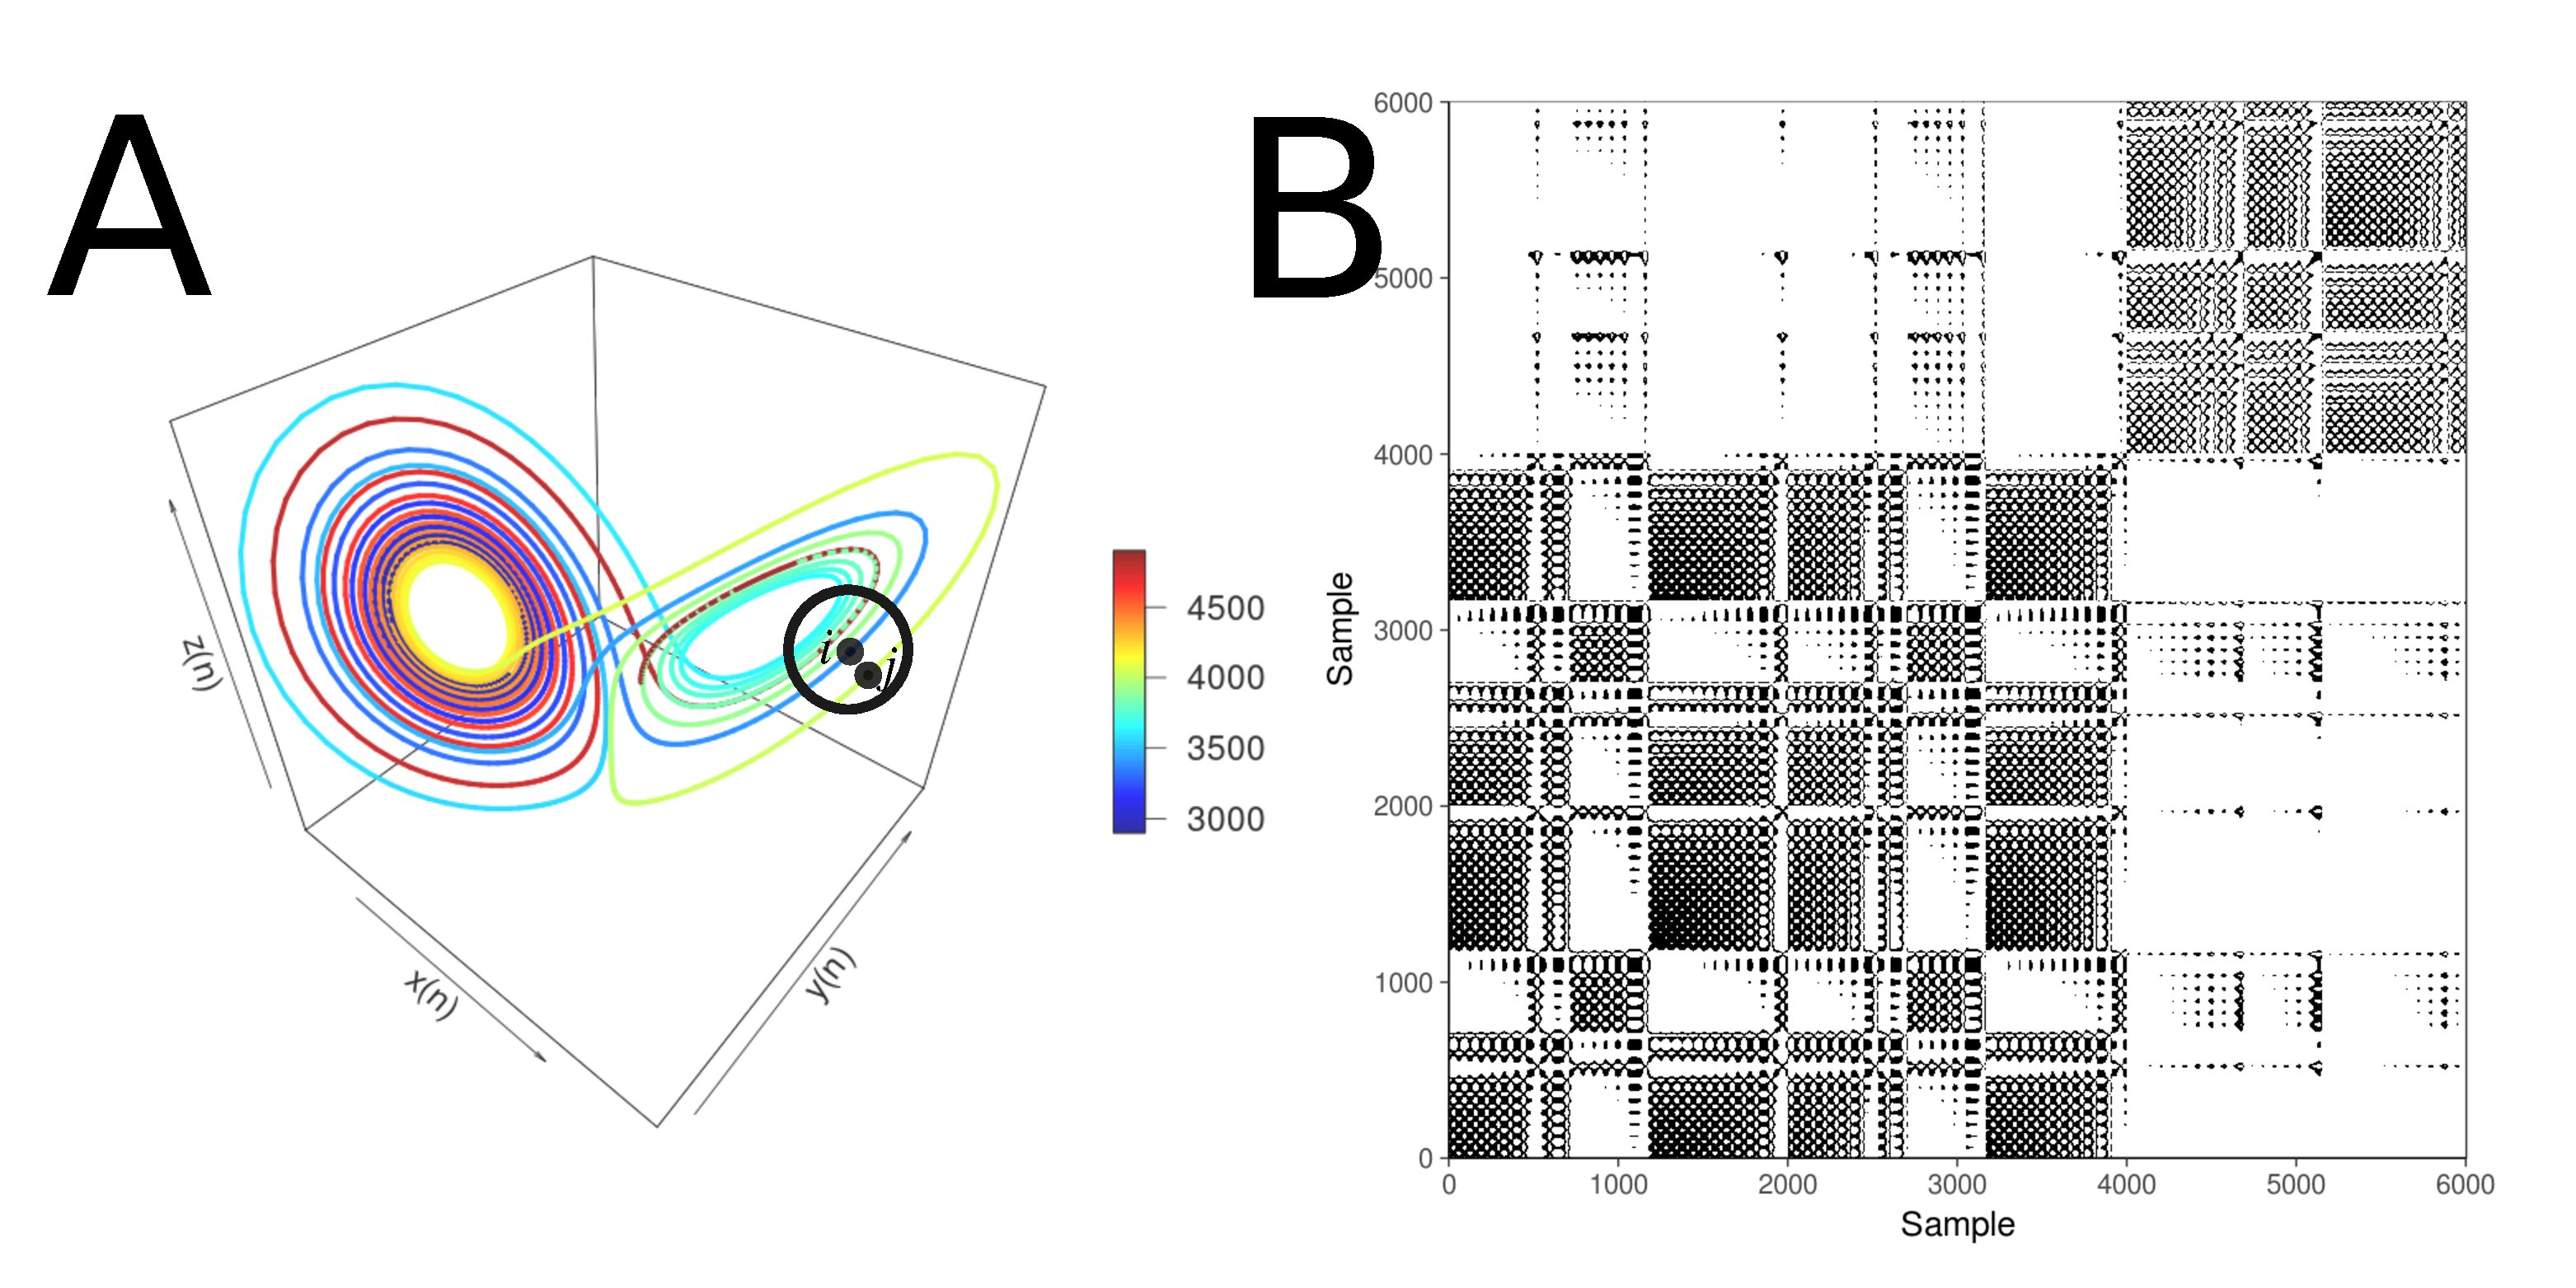
\includegraphics[width=1.0\textwidth]{fig_3_05}
    \caption
	[Recurrence Plots]{
	{\bf Recurrence Plots.} 
	(A) State space of the Lorenz system with controlling parameters 
	($\rho=28, \sigma=10, \beta=8/3$). A point, $j$, in trajectory $X()$ 
	which falls into the neighborhood (black circle) of a given point 
	at $i$ is a recurrent point and is represented as a black dot in 
	the recurrence plot at location $(i, j)$ or white otherwise.
	(B) Recurrence plot using the three components of the Lorenz 
	system and the RP with no embeddings and threshold $\epsilon=5$.
	This figure is adapted from \cite{marwan2015}.
	\R code to reproduce the figure is available at 
	\codelink{
        https://github.com/mxochicale/phd-thesis/tree/master/0_code_data/1_code/4_figs_ch3/fig_3.5/code
	}.
	}
    \label{fig:mrp}
\end{figure}
%%---------------------------------(FIGURE)-------------------------------------

\subsection{Structures of Recurrence Plots}
Pattern formations in RPs can be designated either 
as topology for large-scale patterns or texture for small-scale patterns.
In the case of topology, the following pattern formations are presented:
(i) homogeneous where uniform recurrence points are spread in the RP e.g., 
uniformly distributed noise (Figure~\ref{fig:rp2}A), 
(ii) periodic and quasi-periodic systems where diagonal lines and 
checkerboard structures represent oscillating systems, e.g., sinusoidal 
signals (Figure~\ref{fig:rp2}B), 
(iii) drift where paling or darkening recurrence points away from 
the LOI is caused by drifting systems, 
e.g., logistic map (Figure~\ref{fig:rp2}C), and
(iv) disrupted where recurrence points are presented white areas or 
bands that indicate abrupt changes in the dynamics, e.g. Brownian motion 
(Figure~\ref{fig:rp2}D) \citep{eckmann1987, marwan2015}.
Texture, for small-scale patterns, can be categorised as:
(i) single or isolated recurrence points that represent rare occurring 
states, do not persist for any time or fluctuate heavily,
(ii) dots forming diagonal lines where the length of the small-scale parallel 
lines in the diagonal are related to the ratio of determinism or 
predictability in the dynamics of the system, and
(iii) dots forming vertical and horizontal lines where the length of the 
lines represent a time length where a state does not change or change very 
slowly and the patterns formation represent discontinuities in the signal, and
(iv) dots clustering to inscribe rectangular regions which are related 
to laminar states or singularities \citep{marwan2015}.

%%---------------------------------(FIGURE)-------------------------------------
\begin{figure}
  \centering
    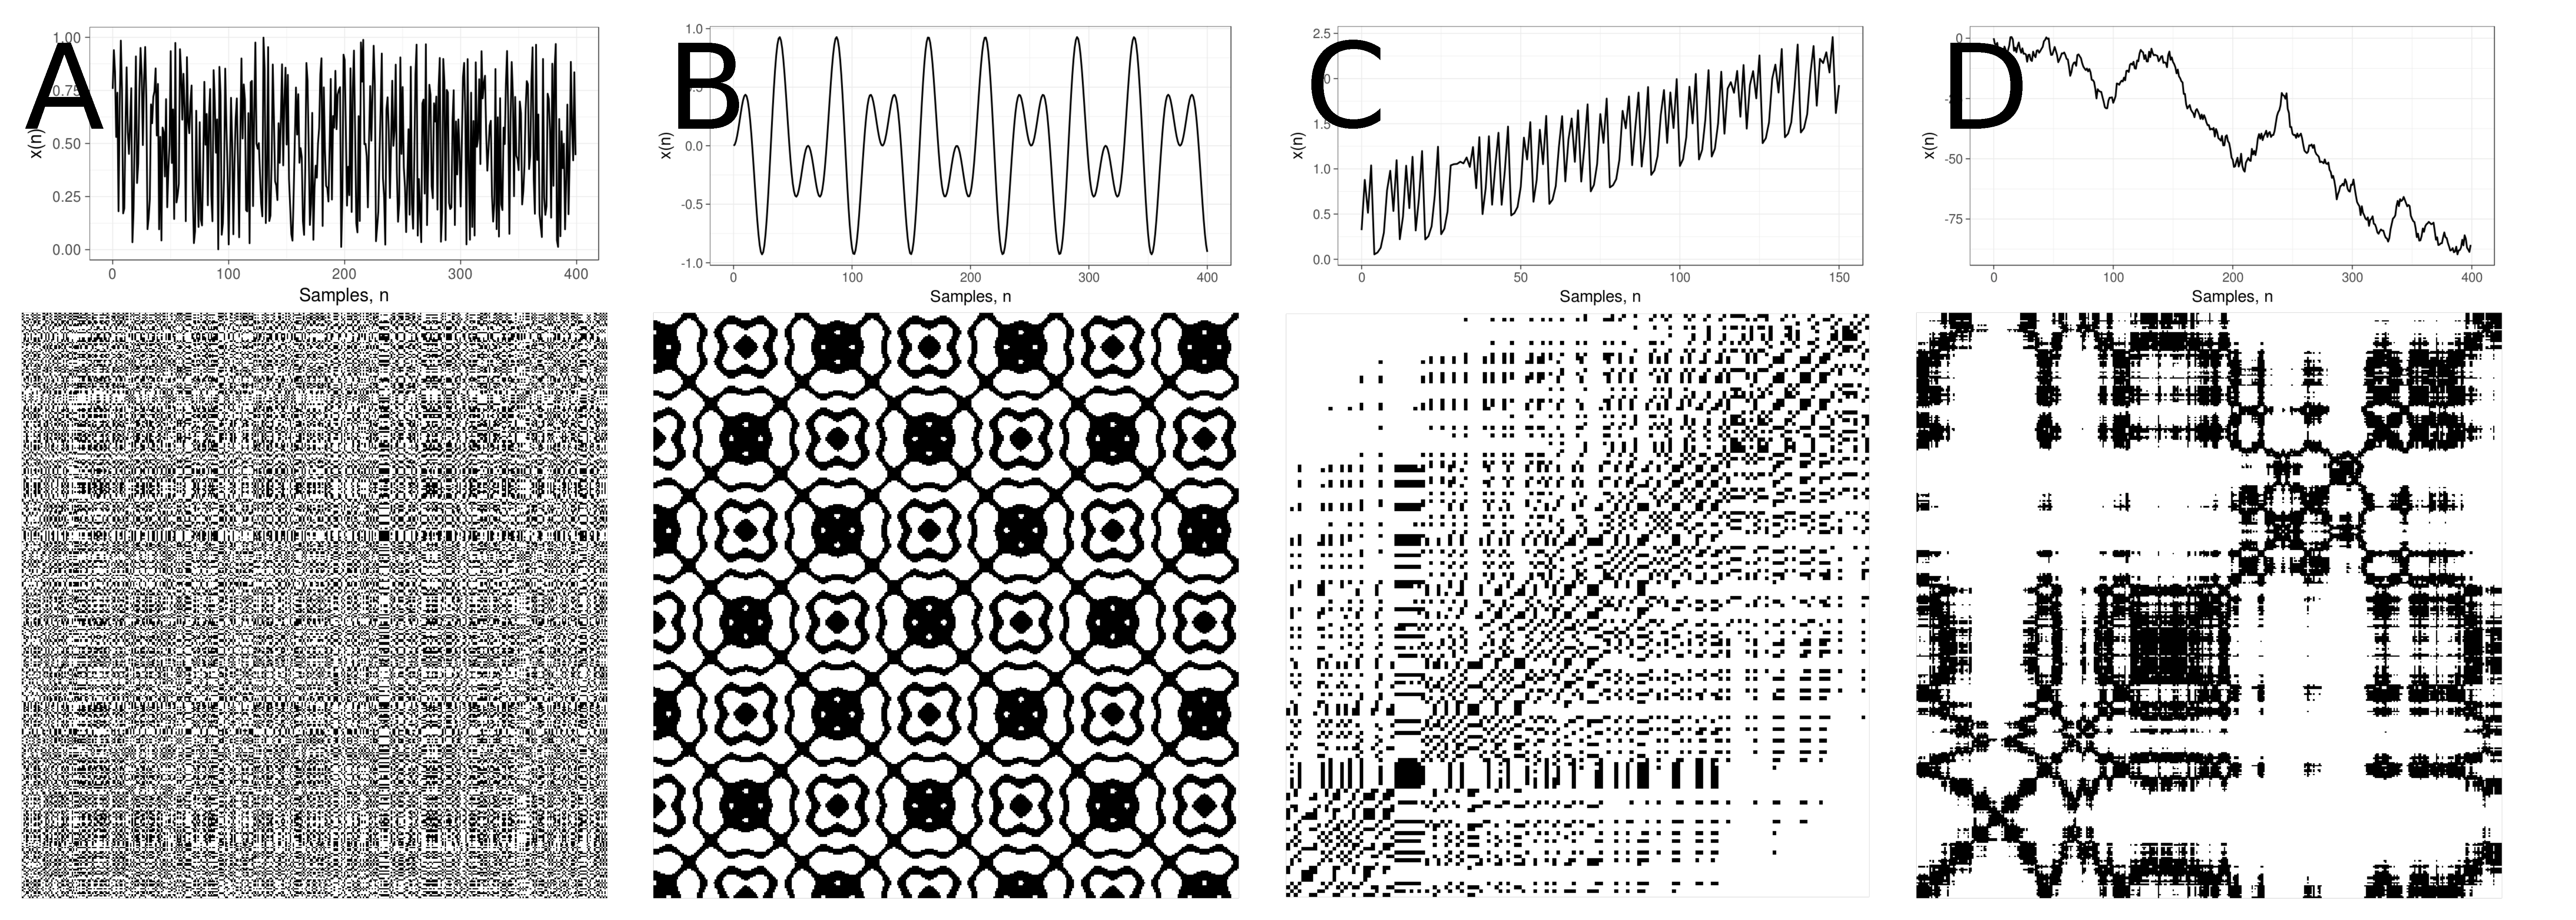
\includegraphics[width=1.0\textwidth]{fig_3_06}
    \caption
	[Patterns in Recurrence Plots]{
	{\bf Patterns in Recurrence Plots.} 
	Time-series with its respective recurrence plots for:
	(A) uniformly distributed noise,
	(B) super-positioned harmonic oscillation 
	($\sin{ \frac{1}{5} t} \sin{ \frac{5}{100}t) }$),
	(C) drift logistic map ($x_{i+1} = 4 x_i (1- x_i) $) corrupted 
	with a linearly increase term ($0.01 i$), and
	(D) disrupted brownian motion  ($x_{i+1} = x_i + 2rnorm(1) $).
	Figure is adapted from \cite{marwan2015}.
	\R code to reproduce the figure is available at 
	\codelink{
	https://github.com/mxochicale/phd-thesis/tree/master/0_code_data/1_code/4_figs_ch3/fig_3.6/code
	}.
	}
    \label{fig:rp2}
\end{figure}
%%---------------------------------(FIGURE)-------------------------------------

Although, the previous pattern descriptions of the structures in the 
RP offer an idea of the characteristics of dynamical systems from 
time-series, these descriptions might be misinterpreted and conclusions might 
tend to be subjective as these require the interpretation of a researcher(s).
Because of that, recurrence quantification analysis (RQA) offers objective
metrics to quantify the visual characteristics of recurrent 
pattern structures in the RP \citep{zbilut1992}.

\section{Recurrence Quantifications Analysis (RQA)} \label{sec:rqa}
\cite{zbilut1992} proposed metrics to investigate the density of recurrence 
points in RPs, then histograms of lengths for diagonal lines in RPs were 
studied by \cite{trulla1996}, then \cite{marwan2008} introduced the term 
Recurrence Quantification Analysis (RQA). 
There are different RQA metrics such as percentage of recurrence, 
percentage of determinism, ratio, Shannon entropy of the 
frequency distributions of the line lengths, maximal line length and 
divergence, trend and laminarity \citep{marwan2007, marwan2015}.
For this thesis, I therefore considered only four RQA metrics 
(i.e. REC, DET, RATIO and ENT) due to their relationship with the 
variables of complexity and predictability from models of movement 
variability \citep{stergiou2006, vaillancourt2002, vaillancourt2003}.

\subsection{Measures of RP based on the recurrence density}
%%%%%%%%%%%%%%%
%(1st variable) 
The percentage of recurrence (REC) or recurrence rate (RR) is defined as
%%********************************[EQUATION]************************************
\begin{equation}
	REC(\epsilon,N)= 
	\frac{1}{N^2 - N} \sum^{N}_{i \neq j = 1} 
	\mathbf{R}^{m}_{i,j}(\epsilon),
\end{equation}
%%********************************[EQUATION]************************************
which enumerates the black dots in the RP excluding the line of identity.
RR is a measure of the relative density of recurrence points in the sparse 
matrix \citep{marwan2015}.
%REC is computed as follow with the nonlinearTseries package \cite{nonlinearTseries} 
%  hist = getHistograms(neighs, ntakens, lmin, vmin)
%  # calculate the number of recurrence points from the recurrence rate. The
%  # recurrence rate counts the number of points at every distance in a concrete
%  # side of the main diagonal.
%  # Thus, sum all points for all distances, multiply by 2 (count both sides) and
%  # add the maindiagonal
%  numberRecurrencePoints = sum(hist$recurrenceHist) + ntakens
%  # calculate the recurrence rate dividing the number of recurrent points at a
%  # given distance by all points that could be at that distance
%  recurrence_rate_vector = hist$recurrenceHist[1:(ntakens - 1)] / ((ntakens - 1):1)
%  # percentage of recurrent points
%  REC = (numberRecurrencePoints) / ntakens ^ 2

\subsection{Measures of RP based on diagonal lines}
%%%%%%%%%%%%%%%
%(2nd variable) 
The percent of determinism (DET) is defined as the fraction of recurrence points
that form diagonal lines and it is determined by
%%********************************[EQUATION]************************************
\begin{equation}
	DET=\frac{\sum^{N}_{l=d_{min}} l H_D{l} }{\sum^{N}_{i,j=1} 
	\mathbf{R}_{i,j}(\epsilon) },
\end{equation}
%%********************************[EQUATION]************************************
where 
%%********************************[EQUATION]************************************
\begin{equation}
	H_D(l) = \sum^{N}_{i,j=1} (1- \mathbf{R}_{i-1,j-1}(\epsilon) ) 
		(1- \mathbf{R}_{i+l,j+l}(\epsilon) ) 
		\prod^{l-1}_{k=0}  \mathbf{R}_{i+k,j+k}(\epsilon)
\end{equation}
%%********************************[EQUATION]************************************
is the histogram of the lengths of the diagonal structures in the RP.

DET can be interpreted as the predictability of the system,
for instance, periodic signals have longer diagonal lines, 
chaotic signals have shorter diagonal lines and 
absent of diagonal lines results from stochastic 
signals \citep{marwan2007, marwan2015}. 
Similarly, DET is considered as a measurement for 
the organisation of points in RPs \citep{iwanski1998}. 
%percent determinism (DET) is computed as follow with the nonlinearTseries package \cite{nonlinearTseries}  
% calculateDiagonalParameters = function(ntakens, numberRecurrencePoints,
%                                       lmin = 2, lDiagonalHistogram,
%                                       recurrence_rate_vector, maxDistanceMD) {
%  #begin parameter computations
%  num = sum((lmin:ntakens) * lDiagonalHistogram[lmin:ntakens])
%  DET = num / numberRecurrencePoints

%%%%%%%%%%%%%
%(X variable) 
RATIO is defined as the ratio between DET and REC and it is calculated from 
the frequency distributions of the lengths of the diagonal lines.
RATIO is useful to discover dynamic transitions \citep{marwan2015}.
%  diagP = calculateDiagonalParameters(
%    ntakens, numberRecurrencePoints, lmin, hist$diagonalHist,
%    recurrence_rate_vector, maxDistanceMD
%  )
% calculateDiagonalParameters = function(ntakens, numberRecurrencePoints,
%                                       lmin = 2, lDiagonalHistogram,
%                                       recurrence_rate_vector, maxDistanceMD) {
%  #begin parameter computations
%  num = sum((lmin:ntakens) * lDiagonalHistogram[lmin:ntakens])
%  DET = num / numberRecurrencePoints
% 
%
%    RATIO = diagP$DET / REC
%

%%%%%%%%%%%%%%%
%(4th variable) 
ENT is the Shannon entropy of the frequency distribution of the diagonal line 
lengths and it is defined as
%%********************************[EQUATION]************************************
\begin{equation}
	ENT= - \sum^{N}_{l=d_{min}} p(l) \ln{p(l)} \quad where \quad 
		p(l)=\frac{ H_D(l) }{ \sum^{N}_{ l=d_{min} } H_D(l) }.
\end{equation}
%%********************************[EQUATION]************************************
ENT reflects the complexity of the deterministic structure in the system.
For instance, for uncorrelated noise or oscillations, 
the value of ENT is rather small and indicates low complexity of the system,
therefore "the higher the ENT is the more complex the dynamics are" 
\citep[p. 15]{marwan2015}.
%#'  \item \emph{ENTR}: Shannon entropy of the diagonal line lengths distribution
%
%calculateDiagonalParameters = function(ntakens, numberRecurrencePoints,
%                                       lmin = 2, lDiagonalHistogram,
%                                       recurrence_rate_vector, maxDistanceMD) {
%
%  pl = lDiagonalHistogram / sum(lDiagonalHistogram)
%  diff_0 = which(pl > 0)
%  ENTR = -sum(pl[diff_0] * log(pl[diff_0]))
 
\subsection{Some weaknesses and strengths of RP and RQA.} \label{sec:ws_rqa}
One of the main advantages of the use of RP is its capacity to detect 
small modulations in frequency or phase that are not detectable 
when using standard methods e.g. spectral or 
wavelet analysis \citep{marwan2011}.
Nonetheless, RP is a very young field in nonlinear analysis
and many research remains to be done, for instance, 
RP can create different results because of 
different values for embedding parameters and recurrence thresholds
for different size of window length of time-series data 
\citep{marwan2011, eckmann1987}.
Additionally, the selection of recurrence threshold, $\epsilon$, 
can depend on the system that is under analysis. For instance, when studying 
dynamical invariants $\epsilon$ is required to be very small, for trajectory 
reconstruction $\epsilon$ is required to have a large threshold or 
when studying dynamical transition there is little importance about the 
selection of the threshold \citep{marwan2011}. Other criteria for the 
selection of $\epsilon$ is that the recurrence threshold should be five 
times larger than the standard deviation of the observational noise
or the use of diagonal structures within the RP is suggested in order
to find the optimal recurrence threshold for (quasi-)periodic process 
\citep{marwan2011}.

\cite{iwanski1998} highlighted the importance of choosing 
appropriate embedding parameters to compute RQA 
in order to have a better intuition of the nature 
of the structure of time-series data.
In the same investigation, \cite{iwanski1998} pointed out 
that RQA metrics are quantitatively and qualitatively independent of 
embedding dimension. However, with an example, \cite{iwanski1998} 
showed that two dissimilar Recurrence Plots 
(one from the R\"{o}ssler system and 
the other from a varying-period sine wave signal) have got equal 
values for REC (2.1\%) and have got approximately equal values 
for DET (42.9\%, 45.8\%, respectively).

\subsection{3D surface plots of RQA} \label{sec:3d_rqa}
One approach to tackle some of the previously reviewed weaknesses and 
strengths of RP and RQA is the method of \cite{zbilut1992} 
in which 3D surface plots are created with an increase of 
embedding parameters ($m$ and $\tau$). 
\cite{zbilut1992} explored fluctuations and gradual 
changes in the 3D surface plots to provide information 
about the selection of embeddings parameters. 
Similarly, considering the work of \cite{webber2018}, 
\cite{marwan2015} pointed out that the creation 
of 3D surface plots are useful for visual selection of 
recurrence thresholds and embedding parameters 
(see Fig. 1.16 in \cite{marwan2015}). 

With that in mind, I propose a similar graphical approach 
based on the works of \cite{zbilut1992}, \cite{webber2018}, 
and \cite{marwan2015} in order to visualise fluctuations 
and changes of 3D surface plots of RQA.
Hence, four variables are considered to create 3D surface 
plots of RQA for this thesis: 
(i) embedding dimension,
(ii) embedding delay,
(iii) recurrence threshold, and 
(iv) metrics of RQA. 
Figure \ref{fig:fig_37}(A) illustrates a 3D surface plot of RQA ENTR  
with unitary increment of embedding parameters ($m$ and $\tau$)
for recurrence threshold $\epsilon=2.0$.
Then, Figure \ref{fig:fig_37}(A), 
with other variations of recurrence thresholds 
(i.e., $\epsilon=0.2$, $\epsilon=1.0$, $\epsilon=3.0$), 
is used to create Fig \ref{fig:fig_37}(B) where bands 
for values of $\tau$ are concatenated to form a long band
that is embedded into Fig \ref{fig:fig_37}(B) 
(as illustrated by the arrows).
Additionally, five time series with their 3D surface plots of 
RQA ENTR are shown in Figs \ref{fig:fig_37}(C to G)
to illustrate how 3D surface plots of RQA ENTR differ from each other.
%%---------------------------------(FIGURE)-------------------------------------
\begin{figure}
  \centering
    \includegraphics[width=0.95\textwidth]{fig_3_07}
    \caption
	[3D surface plots]{
	{\bf 3D surface plots.} 
	3D surface plots of RQA ENTR incrementing 
	(A) embedding dimensions ($m$ and $\tau$),
	(B) embedding dimensions ($m$ and $\tau$) and
	recurrence threshold ($\epsilon$).
	Four time-series data and their 3D surface plots of 
	RQA Entr for:
	(C) uniformly distribute noise,
	(D) super-positioned harmonic oscillation 
	($\sin{ \frac{1}{5} t} \sin{ \frac{5}{100}t) }$),
	(E) drift logistic map ($x_{i+1} = 4 x_i (1- x_i) $) corrupted 
	with a linearly increase term ($0.01 i$),
	(F) disrupted brownian motion  ($x_{i+1} = x_i + 2rnorm(1) $), and
	(G) $x(t)$ solution of Lorenz system.
	\R code to reproduce the figure is available at 
	\codelink{
	https://github.com/mxochicale/phd-thesis/tree/master/0_code_data/1_code/4_figs_ch3/fig_3.7/code
	}.
	}
    \label{fig:fig_37}
\end{figure}
%%---------------------------------(FIGURE)-------------------------------------

%FIND AN APPROPRIATE PLACE TO PUT THIS PARAGRAPH
%With that in mind, 
%I state that little has been investigated with regards to: 
%(i) the strengthens and weaknesses of different 
%methods of nonlinear analysis for real-world data
%(see Section \ref{nonlieaRealdata} for 
%non-stationary, data length size sampling rate and noise of 
%time-series data with nonlinear analysis), 
%(ii) different models for movement variability where, for instance, 
%not only the model of \cite{stergiou2006} where complexity and 
%predictability variables can characterise movement 
%variability but also it can take into account the dependencies of the 
%task dynamics \citep{vaillancourt2002, vaillancourt2003} (Section 
%\ref{what_to_measure_with_MV}), and 
%(iii) the selection and application of appropriate methods of 
%nonlinear analysis in order to quantify movement variability 
%(Section \ref{which_NT_are_appropriate_to_measure_MV}).
%
%I, therefore, explore, in this thesis, the weaknesses and strengths of 
%the window size of time series, embedding parameters for RSS with UTDE 
%and recurrence threshold for RP and RQA in order to gain a 
%better insight into the underlying time series collected from inertial 
%sensors in the context of human-humanoid imitation activities.


\newpage
\section{Final remarks}
Fundamentals of nonlinear analysis such 
as RSS with UTDE, estimation of embedding parameters with FNN and AMI, RP, 
and four RQA metrics (REC, DET, RATIO, and ENTR) were introduced in this chapter.
It is important to note that this thesis is only focused on
the application of traditional methods (i.e., FNN and AMI) 
to compute embedding parameters.
See Chapter \ref{chapter7} for future work with 
optimal embedding parameters estimation.
Aditionally, some weaknesses and strengths of RP and RQA metrics 
were presented in this chapter in order to explore
issues of real-world time series data.
One of the contributions of this thesis
is the representation of 3D surface plots of RQAs
that exploit the effect of incrementing 
not only embedding parameters \citep{iwanski1998} but also 
recurrence thresholds.
See the following chapters, 
Chapter \ref{chapter4} for introduction of experiments and
Chapters \ref{chapter5} and \ref{chapter6} for results.


